%\vspace{-1ex}
%%%%%%%%%%%%%%%%%%% Section 8 %%%%%%%%%%%%%%%%%%%%%%%
\section{Experiment 1-- Recommendation}
\label{sec-expt1, for recommendation task}

\textbf{Data Source: }The dataset we used to test the performance of GCN is download from Citation Network Dataset ~\cite{Tang:08KDD}. Once we obtain the Citation network, we can generate positive samples by pairing the any two paper that contain citation relationship as the sample and label to train the GCN model. By using margin-based loss, the model can be trained by data that contain citation relationship. Negative samples are randomly generated, we sample a set of 60 negative items (30 percent of them are viewed as hard-negative samples~\cite{pintest}) to be shared by all training examples in each minibatch.

\textbf{Result: }After 500 epochs of training, we plot the loss value and accuracy.
\begin{figure}[!htb]
    \centering
    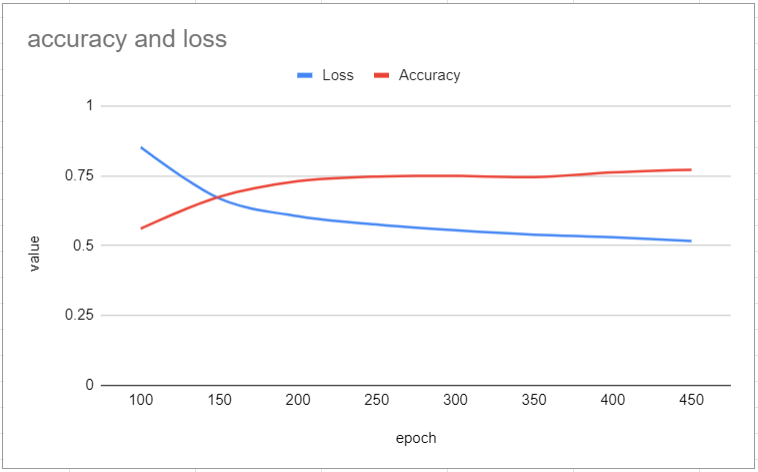
\includegraphics[width=0.48\textwidth]{accandloss.png}
    \caption{Loss value and Accuracy}
    \label{fig:accandloss}
\end{figure}
And an example of the recommendation system is shown in Figure 3. 
\begin{figure}[!htb]
    \centering
    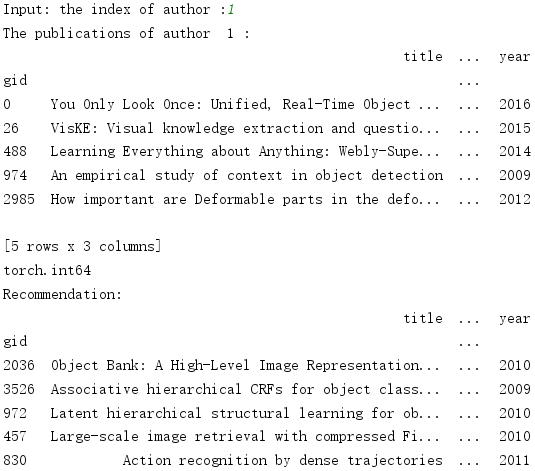
\includegraphics[width=0.48\textwidth]{demo.png}
    \caption{An example of the Recommendation System}
    \label{fig:demo}
\end{figure}
The source code of Experiment 1 to test the proformence of GCN is shown at following link: \url{https://github.com/lovethatcat/EECS_600_deep_learning_final_project}